\chapter{Data Analysis}
\label{ch:data-analysis}

The initial goal of this project was concerned with modeling different infection patterns as influenced by \gls{sirna} mediated gene knockdown. By fitting a \gls{glm} model, using the large set of available cellular features, described in section \ref{sec:scf-data}, as predictor variables and the membership to one of two wells as binary response, it was conjectured to be possible to determine a subset of influential features. Unfortunately, to present data, this has not been possible.

In order the make the substantial amount of single cell data, obtained from several large-scale, high throughput \gls{sirna} screens performed by the InfectX consortium, available to an environment for statistical analysis, an R packages was developed, which is described in chapter \ref{ch:singlecellfeatures}. Building on this crucial piece of infrastructure, the current chapter will explore some of the data analysis that was performed, beginning a short introduction into the models used and continuing with preliminary findings that motivate the investigation of possible normalization schemes. A final outlook on possible improvements will conclude this chapter.

\section{Statistical Models}
Many algorithms for binary classification exist, including decision trees, \glspl{svm}, Bayesian networks, neural networks and \glspl{glm}, some of which have been encountered in previous sections due to their application in infection scoring (see section \ref{sec:infection-scoring}). As neither prediction not classification per se are of main interest, binary logistic regression presents an attractive method due to availability of extensive coefficient and model statistics. Therefore, modeling of \gls{sirna} effects on cellular features is performed, using the glm function provided by the R stats package \citep{RCoreTeam2015}, as well as glmnet belonging to the CRAN package of the same name \citep{Friedman2010a}.

A great many binary comparisons are possible with the given datasets. In order to focus on wells where there is reason to assume they might be biologically interesting, the $n \choose 2$ possible combinations of wells (within a single plate, \tilde 70000 pairs can be formed), are narrowed down using a \gls{pmm} as derived by \cite{Ramo2014}. Of the resulting hit list, several genes are selected and compared to wells containing scrambled \gls{sirna} reagents, which should provide a good choice for establishing background levels. A possible alternative are mock controls but owing to the complete absence of \gls{sirna} molecules, the difference in treatment of cells is only increased and hence it can be conjectured that they provide inferior comparisons.

\subsection{Generalized Linear Models}
Modeling the relationship among variables is one of the most important applications of statistical theory. The study of regression analysis (and the closely related notion of correlation) started to form towards the end of the 19th century with Sir Francis Galton's study of height heredity in humans and his observation of regression towards the mean. Over the next few years, Udny Yule and Karl Pearson cast the developed concepts into precise mathematical formulation, in turn building on work performed by Adrien-Marie Legendre and Carl Friedrich Gauss who developed the method of least squares almost a century earlier \citep{Allen1997}.

A multiple linear regression model can be written in matrix-vector form as
\begin{equation}
  y = X \beta + \epsilon \label{eq:lin-reg}
\end{equation}
where $y \in \R^n$ is the vector of observations on the dependent variable, the design matrix $X \in \R^{n \times p}$ contains data on the independent variables, $\beta \in \R^p$ is the $p$-dimensional parameter vector and the error term $\epsilon \in \R^n$ captures effects not modeled by the regressors.

In order to find unknown coefficients $\beta_i$, the ordinary least squares estimator minimizes the residual sum of squares, the squared differences between observed responses and their predictions according to the linear model.
\begin{subequations}
\begin{align}
  \Hbeta &= \argmin_{\beta} \norm{y - X \beta}^2 \\
         &= (X^T X)^{-1} X^T y \label{eq:ols-estimate}
\end{align}
\end{subequations}
Some assumptions are typically associated with linear regression models that yield desirable attributes for the estimates. None of these restrictions are imposed on the explanatory variables; they can be continuous or discrete and combined as well as transformed arbitrarily. Furthermore, in practice, it is irrelevant whether the covariates are treated as random variables or as deterministic constants. With exception of the field of econometrics it appears that the majority of literature adheres to the latter interpretation and therefore, statements will not explicitly be conditional on covariate values.
\begin{description}
  \item[Linearity.] The relationship between dependent and independent variables is assumed to be linear (after suitable transformations) and individual effects additive. If this cannot be satisfied, a linear model is not suitable.
  \item[Full rank.] For the matrix $X^T X$ to be invertible, it has to have full rank $p$. Therefore $n \leq p$ and all covariates must be linearly independent.
  \item[Exogeneity.] All independent variables should be known exactly i.e. contain no measurement or observation errors as only the mean squared error of the dependent variable is minimized. Additionally, all important causal factors have to be included in the model. Exogeneity implies $\Erw[\epsilon_i] = 0 \forall i$, as well no correlation between regressors and error terms \citep{Hayashi2000}.
  \item[Spherical errors.] This includes both homoscedasticity or constant error variance, $\Erw[\epsilon_i^2] = \sigma^2 \forall i$, and uncorrelated errors $\Erw[\epsilon_i \epsilon_j] = 0 \forall i \neq j$. These two conditions can be written more compactly as $\Var(\epsilon) = \sigma^2I_{n \times n}$.
  \item[Normality.] For the estimated coefficients to gain some additional desirable characteristics, it can be required that the errors $\epsilon_i$ be jointly normally distributed. Together with the above restrictions on expectation and variance, this yields $\epsilon \sim \N_n(0, \sigma^2 I_{n \times n})$.
\end{description}

Violations of these assumptions have varying consequences. In situations of perfect collinearity, the ordinary least squares estimator $\Hbeta$ as defined in \eqref{eq:ols-estimate} does not exist. Recovering such a situation is possible by using a generalized matrix inverse (for example the Moore--Penrose pseudoinverse) or by dropping the corresponding variables. High correlation inflates coefficient variances, which may be countered by employing a regularization scheme like ridge regression. Omitting a variable that is both correlated with dependent variables and has an effect on the response (a nonzero true coefficient) will introduce bias in the parameters. The method of instrumental variables can help to produce an unbiased estimator.

The assumption of spherical errors ensures that the least squares estimator is the best linear unbiased estimator in the sense that it has minimal variance among all linear unbiased estimators. Heteroscedasticity and autocorrelation do not yield biased coefficient estimates but can introduce bias in \gls{ols} estimates of variance, causing inaccurate standard errors. Such a situation calls for generalized least squares estimation, for example weighted least squares when the data is not homoscedastic ($\sigma^2$ is vector-valued but off-diagonal elements of $\Var(\epsilon)$ are zero), or feasible generalized least squares which can be applied in case of heteroscedasticity and\slash or correlation between errors. Whenever the condition of spherical errors does not hold, \gls{ols} is inefficient and generalized least squares estimators have smaller variance.

Finally, normality provides the framework necessary for applying common hypothesis testing, yielding t-statistics, p-values and confidence intervals for coefficients, as well as an F-statistic for the model as a whole. Furthermore, under normality assumptions, the \gls{ols} estimator and \gls{mle} coincide. Quantile regression and other forms of robust regression, such as M estimators may restore validity of inference when errors do not follow a normal distribution.

Modeling data to a dichotomous response variable with \gls{ols} methodology, while readily possible, often is a bad choice due to violations of several of the above assumptions. First of all, normal distributions are continous with support $x \in \R$ and thusly a categorical variable cannot be normally distributed. Homoscedasticity does not hold as well as can easily be seen in a geometric argument: any line with nonzero slope, fitted to a set of $Y$ with $Y_i \in \{0,1\}$, will produce residuals that vary linearly. Finally and perhaps most importantly, a linear model is unsuitable due to there being no constraints on the range of fitted values. While this could be dealt with, the concept of additivity within this context raises questions of its own when fitted values are thought of as probabilities. Linear behavior throughout the range of 0 (impossible) to 1 (certain) makes no sense for most practical applications, as typically, some flattening is expected when approaching either end of the spectrum.

In view of the above considerations it becomes clear that some sort of extension to ordinary linear regression in needed in order to deal with binary response variables. A theory, unifying several previously separately treated statistical models, including linear regression, \gls{anova}, logistic regression, Poisson regression and multinomial response, as \acrfullpl{glm}, was developped by John Nelder and Robert Wedderburn in the early 1970's \citep{Nelder1972}. Much of this section is based on that work.

In order to accommodate the newly added extensions, the classical linear model is rewritten as

\begin{equation}
  \Erw[Y] = \mu \text{ where } \mu = X \beta,
\end{equation}

yielding a three-part specification, consisting of

\begin{enumerate}[label=(\alph*)]
  \item the \textit{random component}; $Y$ is distributed according to a member of the exponential family,\footnote{Many of the most commonly used distributions belong to the exponential family, including but not restricted to Bernoulli, binomial, Poisson, exponential and normal distributions. Common to all members, the probability density function can be written as
  \begin{equation}
    f(x;\theta) = h(x) e^{\theta^\intercal T(x)-A(\theta)}
  \end{equation}
  where $\theta$ is the vector of paramteters, $T(x)$ the vector of sufficient statistics, $A(\theta)$ the cumulant generating function and $h(x)$ the base measure. In case of the Bernoulli distribution
  \begin{equation}
    f(k;\pi) = \pi^k (1-\pi)^{1-k}\label{eq:bern-pmf}
  \end{equation}
  this gives $h(k) = 1$ $T(k) = k$, $\theta = \log\frac{\pi}{1-\pi}$ and $A(\theta) = \log(1+e^\theta)$. Restricting \glspl{glm} to exponential family distributions makes it possible to stay within the framework of maximum likelihood parameter estimations, as given this restriction, \gls{mle} yields the best parameter estimator with respect to minimal variance.}
  \item the \textit{systematic component}; a linear predictor is given by $\eta = X\beta$,
  \item and the \textit{link} between random and systematic components, expressed as the link function $g(\cdot)$, such that $\eta = g(\mu)$; in case of normally distributed Y, $\mu = \eta$ (identity link).
\end{enumerate}

\renewcommand{\arraystretch}{2}
\setlength{\tabcolsep}{0.2em}
\begin{table}
  \centering
  \caption[Link functions of common univariate distributions of the exponential family.]{Common univariate distributions of the exponential family alongside mean and canonical link functions.}
  \label{tab:glm-links}
  \footnotesize
  \begin{tabular}{L{0.18\linewidth}L{0.18\linewidth}L{0.18\linewidth}L{0.18\linewidth}L{0.18\linewidth}}
    Distribution &
      Support &
      Link name &
      Link function &
      Mean function \\
    \hline 
    Normal &
      $(-\infty, +\infty)$ &
      identity &
      $\eta = \mu$ &
      $\mu = X\beta$\\
    Poisson &
      $\{0, 1, 2, \dotsc\}$ &
      log &
      $\eta = \log(\mu)$ &
      $\mu = e^{X\beta}$\\
    Binomial &
      $\{0, 1, \dotsc, N\}$ &
      logit &
      $\eta = \log\left(\frac{\mu}{1-\mu}\right)$ &
      $\mu = \frac{e^{X\beta}}{1+e^{X\beta}}$\\
    Gamma &
      $(0, +\infty)$ &
      reciprocal &
      $\eta = -\mu^{-1}$ &
      $\mu = -(X\beta)^{-1}$\\
    Inverse Gaussian &
      $(0, +\infty)$ &
      inverse squared &
      $\eta = -\mu^{-2}$ &
      $\mu = (-2X\beta)^{-1/2}$\\
  \end{tabular}
\end{table}

Mean and canonical link functions for several common univariate distributions belonging to the exponential family are shown in table \ref{tab:glm-links}. Binary response can be written as 
\begin{equation}
  Y_i \mathbin{\sim} \Bern(\pi_i)
\end{equation}
which implies that
\begin{equation}
  \P(Y_i=1) = 1 - \P(Y_i=0) = \pi_i.
\end{equation}
Therefore, $\pi_i$ can be thought of as the probability of one outcome (i.e. success) and its complement ($1-\pi_i$) corresponds to the probability of the other outcome (failure). Each experimental unit that yields one outcome is associated with a vector of independent variables $(x_{i,1}, x_{i,2}, \dotsc, x_{i,p})$ and the goal of regression in this context becomes modeling the relationship between response probability $\pi_i$ and explanatory variables $(x_{i,1}, x_{i,2}, \dotsc, x_{i,p})$. A suitable link function for Bernoulli distributed response, as discussed above, is required to map the unit interval onto the whole real line and preferably be shaped sigmoidally in order accurately describe increasingly likely as well as increasingly unlikely events. Three possibilities are often considered within this context,

\begin{enumerate}[label=(\alph*)]
  \item the \textit{logit} or logistic function
  \begin{equation}
    g(\pi) = \log\left(\frac{\pi}{1-\pi}\right),
  \end{equation}
  \item the \textit{probit} or inverse normal function
  \begin{equation}
    g(\pi) = \Phi^{-1}(\pi),
  \end{equation}
  with $\Phi(\cdot)$ denoting the cumulative distribution function of the normal distribution,
  \item and the \textit{complementary log-log} function
  \begin{equation}
    g(\pi) = \log\left(-\log(1-\pi)\right).
  \end{equation}
\end{enumerate}

All three functions are continuous and increasing on $(0,1)$ and the first two are symmetric in the sense that $g(\pi) = -g(1-\pi)$, while the third is not. Using a logit link function, the probability of a positive response can therefore be written as
\begin{equation}
  \pi_i = \frac{e^{x_i^\intercal \beta}}{1+e^{x_i^\intercal \beta}}
\end{equation}
and the model is, slightly rearranged, stated as
\begin{equation}
  \log\left(\frac{\pi_i}{1-\pi_i}\right) = x_i^\intercal \beta = \sum_{j=1}^p x_{i,j}\beta_j.\label{eq:log-model}
\end{equation}

where $x_i$ is shorthand for the $i$-th row $(x_{i,1}, x_{i,2}, \dotsc, x_{i,p})$ of the design matrix $X$. Consequently, of a unit change in a covariate $x_{i,j}$ will increase the corresponding probability log-odds by a multiplicative factor $\exp(\beta_j)$, as can easily be seen by exponentiating expression \ref{eq:log-model}.

The likelihood of a set of parameter values $\pi$, given the data $y_i$, is equal to the probability of the data, given the parameters. Hence, in a logistic regression model (see expression \ref{eq:bern-pmf} for the probability mass function of a Bernoulli distribution), we have

\begin{subequations}
\begin{align}
  L(\beta; y) = \P(y; \beta) &= \prod_{i=1}^n \pi_i^{y_i} (1-\pi_i)^{1-y_i} \label{eq:lik-any} \\
  &= \prod_{i=1}^n \frac{e^{x_i^\intercal \beta y_i}}{1+e^{x_i^\intercal \beta}} \label{eq:lik-logit}
\end{align}
\end{subequations}

and expressed, for reasons of convenience, as log-likelihood

\begin{subequations}
\begin{align}
  l(\beta; y) &= \sum_{i=1}^n y_i \log(\pi_i) + (1-y_i) \log(1-\pi_i) \label{eq:loglik-any} \\
  &= \sum_{i=1}^n x_i^\intercal \beta y_i -  \log\left(1+e^{x_i^\intercal \beta}\right). \label{eq:loglik-logit}
\end{align}
\end{subequations}

Both expressions \ref{eq:lik-logit} and \ref{eq:loglik-logit} are derived using the logit link function but any other of the proposed links can be used to substitute $\pi_i$ in equations \ref{eq:lik-any} and \ref{eq:loglik-any}. In order to find the maximum likelihood estimates
\begin{equation}
\Hbeta = \argmax_{\beta} l(\beta; y), 
\end{equation}

the first derivative of $l(\beta; y)$ with respect to $\beta_j$ in required.

\begin{subequations}\label{eq:firstder}
\begin{align}
  \frac{\partial l(\beta)}{\partial \beta_j} &= \sum_{i=1}^n \frac{y_i - \pi_i}{\pi_i (1-\pi_i)} \frac{d \pi_i}{d \eta_i} \frac{\partial \eta_i}{\partial \beta_j} \label{eq:firstder-any} \\
  &= \sum_{i=1}^n \left(y_i - \frac{e^{x_i^\intercal \beta}}{1+e^{x_i^\intercal \beta}}\right) x_{i,j} \label{eq:firstder-logit}
\end{align}
\end{subequations}

Again, \ref{eq:firstder-logit} is obtained from \ref{eq:firstder-any} by using a logit link, and consequently substituting 

\begin{equation*}
  \frac{d \pi_i}{d \eta_i} = \frac{-e^{-\eta_i}}{(1+e^{-\eta_i})} \text{,\ \ } \eta_i = x_i^\intercal \beta \text{\ \ and\ \ } \frac{\partial \eta_i}{\partial \beta_j} = x_{i,j}.
\end{equation*}

The log-likelihood maximum is found by setting the first derivatives in \ref{eq:firstder} to zero and solving for $\beta$. No closed form solutions to the resulting equations exist and therefore numerical algorithms such as Newton-Raphson are usually used, which can be formulated as an iteratively re-weighted least squares regression problem. Newton's method attempts to find the root $x_r$ of a differentiable function $f(x)$ by starting with an initial guess $x_0$ and iterating

\begin{equation}
  x_{n+1} = x_n - \frac{f(x_n)}{f^\prime(x_n)}.
\end{equation}

When a good initial guess is made and some restrictions on $f(x)$ apply, the rate of convergence is quadratic\footnote{Given a function$f(x)$, that is three-times differentiable in an interval $I^\ast= [a,b]$ such that $a < x_r < b$ and $f^\prime(x_r) \neq 0$, there exists an interval $I = [x_r-\delta, x_r+\delta]$, with $\delta > 0$ for which every $x_0 \in I$ converges quadratically towards $x_r$ \citep{Schwarz2006}.} and even if certain conditions do not hold, or the starting point is not suitably chosen, the algorithm may still converge towards the root. Returning to maximum likelihood notation of expression \ref{eq:firstder}, a Newton-Raphson iteration can be written as

\begin{equation}
  \beta^{(n+1)} = \beta^{(n)} - \frac{l^\prime(\beta^{(n)})}{l^{\prime\prime}(\beta^{(n)})}.\label{eq:nr-loglik}
\end{equation}

The second derivative of the log likelihood with respect to $\beta$, as needed in \ref{eq:nr-loglik} is

\begin{equation}
  \frac{\partial^2 l(\beta)}{\partial \beta_j\partial \beta_k} = -\sum_{i=1}^n \frac{1}{\pi_i (1-\pi_i)} \left(\frac{d \pi_i}{d \eta_i}\right)^2 \frac{\partial \eta_i}{\partial \beta_j} \frac{\partial \eta_i}{\partial \beta_k},
\end{equation}

which, in matrix form, can be written as

\begin{equation}
   \frac{\partial^2 l(\beta)}{\partial \beta\partial \beta^\intercal} = -X^\intercal W X,
\end{equation}

with the $n \times n$ diagonal matrix $W$

\begin{equation*}
  W = \diag\left\{\frac{1}{\pi_i (1-\pi_i)} \left(\frac{d \pi_i}{d \eta_i}\right)^2\right\} \text{,\ \ as\ \ } \frac{\partial \eta_i}{\partial \beta_j} = x_{i,j} \text{\ \ and \ \ } \frac{\partial \eta_i}{\partial \beta_k} = x_{i,k}.
\end{equation*}

In the case of logistic regression, $W$ simplifies to $w = \diag\{\pi_i (1-\pi_i)\}$ and $l^\prime(\beta)$ can be written in matrix form as $l^\prime(\beta) = X^\intercal (y - \pi)$.

Using these results, expression \ref{eq:nr-loglik} can be rewritten as

\begin{equation}
  \beta^{(n+1)} = \beta^{(n)} + \frac{X^\intercal (y - \pi)}{X^\intercal W X},
\end{equation}

which is iterated until the updates become smaller than a threshold, at which point convergence is said to have been reached.

% finish with linking to irls (see esl, p120)

%\subsection{Regularization}
%Two regularization schemes, ridge regression and lasso regression, will be introduced very briefly due to their availability in glmnet.
% esl p61

\subsection{Parallel Mixed Model}
As a way of exploiting replication, typically involved in \gls{sirna} screening, at the level of individual sequences, different sequences targeting the same gene and as is the case for InfectX, different treatments in the form of varying pathogens, \citeauthor{Ramo2014} developed a \gls{pmm}, capable of gaining statistical power from structural parallelism. All following remarks are adapted from the referenced publication and the topic is only outlined briefly for completeness sake. The interested reader is directed to \cite{Ramo2014} for more information. The proposed model is written as

\begin{equation}
  y_{pgs} = \mu_p + a_g + b_{pg} + \epsilon_{pgs},
\end{equation}

where $y_{pgs}$ represents the per-well phenotype (e.g. infection score), which is described as the sum of a fixed effect $\mu_p$ for pathogen $p$, as well as random effects $a_g$ for gene $g$, $b_{pg}$, a correction for gene $g$ within pathogen $p$, and an error term $e_{pgs}$. The overall effect of gene knockdown $g$ under pathogen treatment $p$ therefore is 



\begin{knitrout}
\definecolor{shadecolor}{rgb}{0.969, 0.969, 0.969}\color{fgcolor}\begin{figure}

{\centering 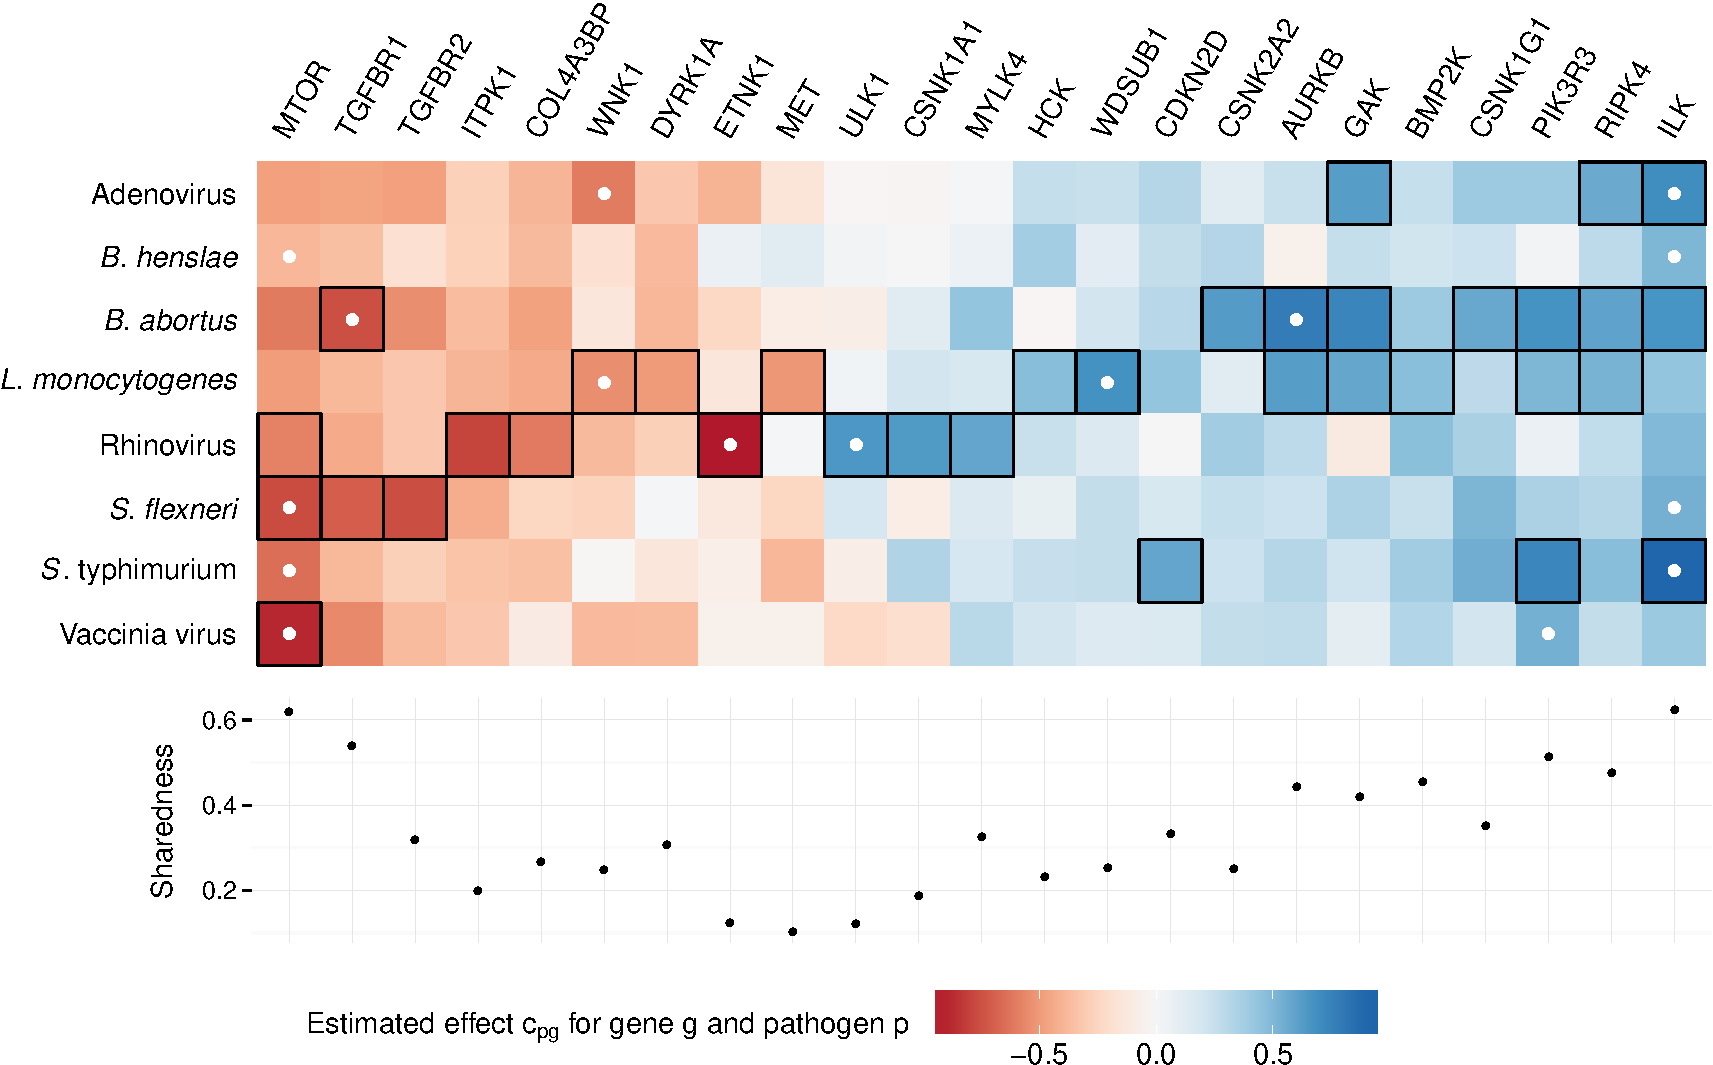
\includegraphics[width=.95\linewidth]{figures/R/pmm-pmm-heatmap-1} 

}

\caption[Heatmap plot showing significant genes for InfectX kinome screens as determined by pmm.]{A heatmap plot as produced by the Bioconductor package pmm, which displays all genes that were determined to be significant hits (FDR < 4; indicated by black borders) for at least one pathogen. Genes are ordered by average c\textunderscript{pg} values and both extrema are marked with white dots, while the sharedness score is shown as a scatterplot below. All available kinome screens were taken into consideration.}\label{fig:pmm-heatmap}
\end{figure}


\end{knitrout}




\begin{equation}
  c_{pg} = a_g + b_{pg},
\end{equation}

and a positive estimated effect corresponds to enhanced infection levels, whereas a negative $c_{pg}$ value indicates reduced infectivity. Random effects are distributed as $a_g \mathbin{\sim} \N(0, \sigma_a^2)$, $b_{pg} \mathbin{\sim} \N(0, \sigma_b^2)$ and $\epsilon_{pgs} \mathbin{\sim} \N(0, \sigma_\epsilon^2)$, and estimation is carried out by the CRAN package lme4, using restricted maximum likelihood. Hits are selected according to an estimated local \gls{fdr} which assumes that a mixture of two distributions corresponding to genes that are no hits ($f_0$) and genes that actually are hits ($f_1$), generates the overall distribution. Furthermore, it is assumed that $f_0 \mathbin{\sim} \N(0, \sigma_a^2+\sigma_b^2)$ and $f_0 \mathbin{\sim} \N(\theta, \sigma_a^2+\sigma_b^2)$, i.e. the two distributions are identical except for a shift in mean by $\theta$. The overall distribution can be expressed as $f(c_{pg}) = \pi_0 f_0(c_{pg}) + (1-\pi_0) f_1(c_{pg})$, where $\pi_0$ is the proportion of true hits. Finally, the \gls{fdr} is defined as

\begin{equation}
  q_{pg} = \fdr(c_{pg}) = \frac{\pi_0 f_0(c_{pg})}{f(c_{pg})}
\end{equation}

and represents the probability that the effect for a given gene and pathogen is a false discovery. Figure \ref{fig:pmm-heatmap} displays a visualization obtained by applying the PMM package (available on Bioconductor) to kinome-wide InfectX screens. Color-coding corresponds to estimated $c_{pg}$ effects and only genes are included where the estimated \gls{fdr} is below 0.4 for at least one pathogen (indicated by black borders). Centered white dots indicate the maximum and minimum $c_{pg}$ value for each pathogen. For each gene, a sharedness score is displayed as well. This quantity is defined as

\begin{equation}
  s_g = \frac{1}{2} \left(\left(1-\frac{1}{P}\sum_{p=1}^P q_{pg}\right) + \frac{\sum_{p=1}^P \mathds{1}_{q_{pg} < 1}}{P}\right)
\end{equation}

and quantifies how common a hit gene is among pathogens by quantifying both the extent of downward shift from 1 of the mean $q_pg$ value (over all $P$ pathogens), as well as the fraction of pathogens that contribute $q_pg < 1$ instances.

\section{Preliminary Findings}
% glm perfect separation, bootstrapped stuff
\section{Data Normalization}
%\section{Modeling Approach}
\section{Outlook and Conclusion}